\documentclass[12pt]{article}

\input preamble

\title{Principles of Parallel Architecture\\
Synchronization}
\author{Xitong Liu \\
xliu@ece.udel.edu}

\begin{document}

\maketitle

\section{Synchronization Primitives}
\subsection{Description}
The objective of this part is to learn how to write fast synchronization 
primitives. And what are the key characteristics that they expose.

Research what atomic operations can be used on cluster. A few suggestions 
read the file \texttt{/proc/cpuinfo} on cluster, and read the following 
website:

\texttt{http://gcc.gnu.org/onlinedocs/gcc-4.1.2/gcc/Atomic-Builtins.html}

Describe briefly the atomic operations and its syntax.

\subsection{Answer}
These build-in functions were provided by GCC to implement the atomic 
operation on Intel Intanium Processors. All these function will be 
translated to Intel Intanium Processor-specific assembly intrinsics.

There are four groups of functions. The first group were
\begin{verbatim}
type __sync_fetch_and_add (type  *ptr, type value, ...)
type __sync_fetch_and_sub (type *ptr, type value, ...)
type __sync_fetch_and_or (type *ptr, type value, ...)
type __sync_fetch_and_and (type *ptr, type value, ...)
type __sync_fetch_and_xor (type *ptr, type value, ...)
type __sync_fetch_and_nand (type *ptr, type value, ...)
\end{verbatim}
in which the value at \texttt{*ptr} will be fetched first and the associated 
operation (e.g. add, sub, or, and) will be applied. The operands for the
operation are the value at \texttt{*ptr} and passed-in \texttt{value} as 
parameter. The result of the operation will be stored at \texttt{*ptr}. The 
old value at \texttt{*ptr} will be returned then.

The second group were
\begin{verbatim}
type __sync_add_and_fetch (type  *ptr, type value, ...)
type __sync_sub_and_fetch (type *ptr, type value, ...)
type __sync_or_and_fetch (type *ptr, type value, ...)
type __sync_and_and_fetch (type *ptr, type value, ...)
type __sync_xor_and_fetch (type *ptr, type value, ...)
type __sync_nand_and_fetch (type *ptr, type value, ...)
\end{verbatim}
They are basically the same with the first group. The only difference between 
them is that the second group functions apply the operation on the operands 
first, and the new value at \texttt{*ptr} will be returned.

The third group were
\begin{verbatim}
bool __sync_bool_compare_and_swap (type  *ptr, type oldval type newval, ...)
type __sync_val_compare_and_swap (type *ptr, type oldval type newval, ...)
\end{verbatim}
These two function perform an atomic compare and swap. If the current value of 
\texttt{*ptr} is \texttt{oldval}, then write \texttt{newval} into \texttt{*ptr}.

The last group were
\begin{verbatim}
__sync_synchronize (...)
type __sync_lock_test_and_set (type  *ptr, type value, ...)
void __sync_lock_release (type *ptr, ...)
\end{verbatim}
The first function performs a full memory barrier. The last two functions were 
not traditional test-and-set operations, but rather an atomic exchange operation. 
The second function writes value into \texttt{*ptr}, and returns the previous 
contents of \texttt{*ptr} and the third function write the constant 0 to 
\texttt{*ptr}.

\end{document}

\begin{comment}
\begin{figure}[h!]
	\begin{center}
		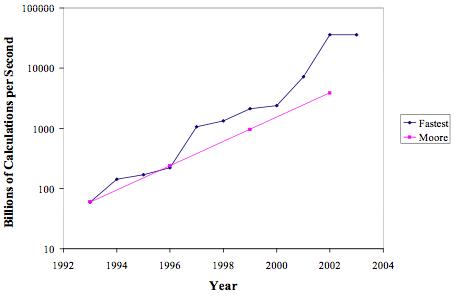
\includegraphics[width=0.7\textwidth, angle=0]{fatest.png}
		\caption{\label{fig:fatest}Fatest SuperComputer in the world}
	\end{center}
\end{figure}
\end{comment}